\subsection{Ethereum}

Ethereum is a decentralised computing platform, that runs small programs called \textit{smart contracts}. It builds on similar concepts as Bitcoin, such as blockchain and consensus based on proof-of-work. Smart contracts are written in Ethereum Virtual Machine bytecode and executed by the \acrfull{evm}. Ethereum was proposed in 2013 by cryptocurrency researcher Vitalik Buterin and was launched in an \acrlong{ico}\footnotemark  in 2014. 
% 
\footnotetext{In an \acrfull{ico} a small percentage of cryptocurrency is sold to a small percentage of backers in a capital-raising process. \url{https://www.investopedia.com/terms/i/initial-coin-offering-ico.asp}, accessed 10-04-2018}
% 
It is currently developed by a Swiss non-profit organisation \textit{Ethereum Foundation}.\footnotemark
% 
\footnotetext{\url{https://www.ethereum.org/foundation}, accessed 10-04-2018}

\subsubsection{Principle of operation}
While in Bitcoin the blockchain only keeps track of unspent transaction outputs, Ethereum blockchain is more complex. It does involve transactions of own currency, which is called \textit{Ether}, but it goes further and introduces other functionality. It is better described as ``\textit{a state machine, where the distributed nodes maintain a shared view of a global state}''~\cite{Tikhomirov2018Ethereum:Perspectives}. Ethereum users issue transactions, which are distributed among the nodes and which change the state of said state machine. Users can make transactions for one of the following reasons~\cite{Atzei2017ASoK}:
\begin{itemize}[noitemsep]
    \item Create a smart contract.
    \item Invoke a function of a smart contract.
    \item Transfer Ether to a smart contract or to another user.
\end{itemize}

Since \acrshort{evm} bytecode is a Turing complete language~\cite{Tikhomirov2018Ethereum:Perspectives, Atzei2017ASoK, Dannen2017IntroducingSolidity}, smart contracts could possibly perform wide variety of computations. However, this has limited use in practice. Every time a transaction invokes a smart contract function, all nodes that observed this transaction, will run the function of the smart contract at once. This redundancy is a desired feature of a decentralised computing platform, such as Ethereum~\cite{EthereumCommunityEthereumDocumentation}, but could lead to a lot of wasted resources, if large quantities of useless computations are to be performed on many nodes at the same time.

To prevent \acrfull{dos} attacks caused by smart contracts containing endless loops or very intense computations, there is a price associated with every atomic instruction, which in Ethereum terminology is called \textit{gas}. When a transaction is made, it must specify the maximum amount of gas that can be used to compute the code of a smart contract. If the code of the smart contract includes many computations, the contract will use more gas. If it does not finish computing before it reaches the maximum amount of gas, any changes made by the computations will be reverted, but the gas will not be returned. To prevent this from happening, users might set the maximum gas limit high enough, so that the smart contract will not run out of gas during its operation. However, the code of the smart contract is computed on all the nodes participating in the network. To avoid all these nodes carrying out huge amount of (potentially useless) computation, the gas is not free and needs to be purchased\footnotemark. 
% 
\footnotetext{The term \textit{gas} was not chosen coincidentally. It is supposed to resemble the gas we put in our car. The metaphor is as follows: \textit{Our smart contract is the car and the computations performed by the smart contract is the distance driven. If we want to drive further, the car will use more gas. We pay some price per litre of gas, when we stop at the gas station. If we want to drive further, we need to purchase more gas.}}

The gas is purchased at the time when a transaction is made and its price is determined by the free market~\cite{EthereumCommunityEthereumDocumentation}. If an attacker was to invoke an endless loop in a smart contract, the loop would only execute while having enough gas to do so. To spam the network with computationally intense transactions, an attacker would need to purchase high amount of gas and the attack would become too expensive~\cite[p.5]{Atzei2017ASoK}.

\subsubsection{Proof of work}
Similarly as Bitcoin, Ethereum uses proof-of-work to reach consensus. Nodes verify incoming transactions and include them together in a block. This block is then hashed using Ethash, a memory-intensive hash function~\cite[p. 211]{Tikhomirov2018Ethereum:Perspectives}. The hash of the block needs to be below target value to be considered valid. Similarly as in Bitcoin, this process is called mining.  A memory intensive hash function was chosen to target \acrshort{gpu} as the main mining hardware, in order to avoid high barriers for entry. Since \acrshort{gpu} market segment is mainly targeted at other areas, such as gaming or high-performance computing, powerful hardware is already available at the market\footnotemark. The target value for the block hash is adjusted regularly to keep average block production speed constant~\cite{Tikhomirov2018Ethereum:Perspectives}.
% 
\footnotetext{In Bitcoin and other currencies, specialised mining hardware, also referred to as \acrfull{asic} is mainly used for Bitcoin mining. The cost of such hardware and economies of scale make it difficult for small miners to enter the market, therefore weakening one of the main advantages of Bitcoin -- decentralisation~\cite{Tikhomirov2018Ethereum:Perspectives}.}

\subsubsection{Transactions and accounts}
There are two types of accounts defined in Ethereum:
\begin{itemize}[noitemsep]
    \item \textit{\acrfull{eoa}}. \acrshort{eoa}s are accounts controlled by a public-private key-pair that have a non-zero Ether balance. \acrshort{eoa}s can send transactions.~\cite{EthereumCommunityEthereumDocumentation}
    \item \textit{Contract account}. Contract account is an account that has code associated with it. It can run its code and maintain its internal state. It can communicate with other contracts by sending objects called \textit{messages}. Execution of contract's code is triggered by an incoming transaction or a message~\cite{EthereumCommunityEthereumDocumentation}.
\end{itemize}

\subsubsection{Smart contracts}
\acrshort{evm} bytecode is a low-level language, which natively supports cryptographic primitives~\cite{Tikhomirov2018Ethereum:Perspectives}. Smart contracts are usually written in high-level language and are compiled into \acrshort{evm} bytecode before deployment. Most popular language for writing smart contracts is Solidity, which offers JavaScript-like syntax. Solidity compilers exist for various platforms, including a web-based \acrshort{ide}.

Smart contracts usually cannot perform very extensive calculations, as the \acrshort{evm} is not powerful enough and there is a cost associated with all computations performed by the smart contract. Because of this, every smart contract is either used for some sort of financial transaction or at least requires some funds to be transferred to it, so its code can execute. However, smart contract only exists within the realm of the Ethereum blockchain~\cite{JohnWeldon2016BuildingContract}. It can not fetch data from other sources, nor it can directly interact with the user. This is what \textit{decentralised applications}, or DApps cover. A decentralised application its an application, that runs in a decentralised manner (on the blockchain) and uses smart contracts as part of its logic~\cite[p. 149]{Dannen2017IntroducingSolidity}. On top of the smart contracts, a DApp also contains a regular HTML/CSS/JavaScript front end interface. Such interfaces of DApps are known as Web3 and are considered by many~\cite{Dannen2017IntroducingSolidity, LukeHedger2017CrossingDevelopment} as the third generation of Web (the first generation was the original World Wide Web, that hosted static pages; the second generation was defined by web-hosted applications and services~\cite{Dannen2017IntroducingSolidity}). Specialised software is needed to interact with the smart contracts in decentralised application, such as Ethereum browser Mist\footnote{\url{https://github.com/ethereum/mist}, accessed 22-05-2018} or browser extension Metamask\footnote{\url{https://metamask.io/}, accessed 22-05-2018}. Although majority of the DApps are built on Ethereum, there are also some that operate on their own blockchain, other than Ethereum~\cite{AlyssaHertigWhatCoinDesk}. Figure~\ref{fig:web3} illustrates the concept of Web3 and DApps.

\begin{figure}
    \centering
    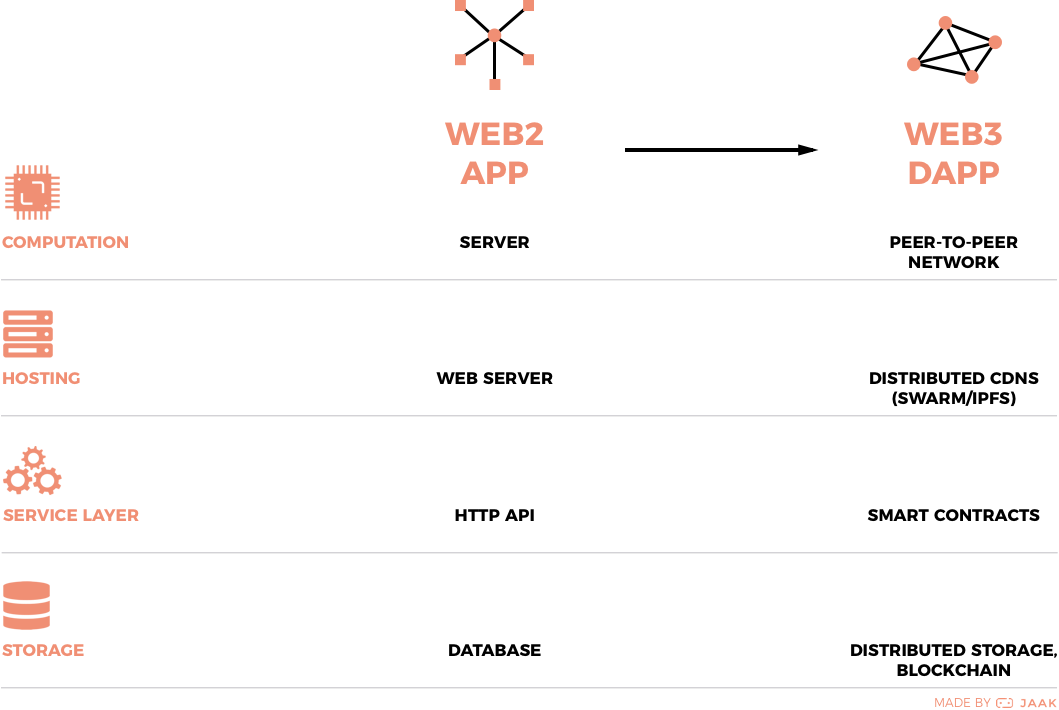
\includegraphics[width=\textwidth]{web3dapp}
    \caption{Comparison of Web2 with Web3. Dicstributed CDNs (Content Delivery Networks), provide hosting to the front end of the DApps (hosting of the HTML/CSS/JavaScript files). Swarm and \acrfull{ipfs} are two exemplary technologies that can provide decentralised such hosting.}
    \label{fig:web3}
\end{figure}